% Options for packages loaded elsewhere
\PassOptionsToPackage{unicode}{hyperref}
\PassOptionsToPackage{hyphens}{url}
\PassOptionsToPackage{dvipsnames,svgnames,x11names}{xcolor}
%
\documentclass[
  letterpaper,
  DIV=11,
  numbers=noendperiod]{scrreprt}

\usepackage{amsmath,amssymb}
\usepackage{iftex}
\ifPDFTeX
  \usepackage[T1]{fontenc}
  \usepackage[utf8]{inputenc}
  \usepackage{textcomp} % provide euro and other symbols
\else % if luatex or xetex
  \usepackage{unicode-math}
  \defaultfontfeatures{Scale=MatchLowercase}
  \defaultfontfeatures[\rmfamily]{Ligatures=TeX,Scale=1}
\fi
\usepackage{lmodern}
\ifPDFTeX\else  
    % xetex/luatex font selection
\fi
% Use upquote if available, for straight quotes in verbatim environments
\IfFileExists{upquote.sty}{\usepackage{upquote}}{}
\IfFileExists{microtype.sty}{% use microtype if available
  \usepackage[]{microtype}
  \UseMicrotypeSet[protrusion]{basicmath} % disable protrusion for tt fonts
}{}
\makeatletter
\@ifundefined{KOMAClassName}{% if non-KOMA class
  \IfFileExists{parskip.sty}{%
    \usepackage{parskip}
  }{% else
    \setlength{\parindent}{0pt}
    \setlength{\parskip}{6pt plus 2pt minus 1pt}}
}{% if KOMA class
  \KOMAoptions{parskip=half}}
\makeatother
\usepackage{xcolor}
\setlength{\emergencystretch}{3em} % prevent overfull lines
\setcounter{secnumdepth}{5}
% Make \paragraph and \subparagraph free-standing
\ifx\paragraph\undefined\else
  \let\oldparagraph\paragraph
  \renewcommand{\paragraph}[1]{\oldparagraph{#1}\mbox{}}
\fi
\ifx\subparagraph\undefined\else
  \let\oldsubparagraph\subparagraph
  \renewcommand{\subparagraph}[1]{\oldsubparagraph{#1}\mbox{}}
\fi

\usepackage{color}
\usepackage{fancyvrb}
\newcommand{\VerbBar}{|}
\newcommand{\VERB}{\Verb[commandchars=\\\{\}]}
\DefineVerbatimEnvironment{Highlighting}{Verbatim}{commandchars=\\\{\}}
% Add ',fontsize=\small' for more characters per line
\usepackage{framed}
\definecolor{shadecolor}{RGB}{241,243,245}
\newenvironment{Shaded}{\begin{snugshade}}{\end{snugshade}}
\newcommand{\AlertTok}[1]{\textcolor[rgb]{0.68,0.00,0.00}{#1}}
\newcommand{\AnnotationTok}[1]{\textcolor[rgb]{0.37,0.37,0.37}{#1}}
\newcommand{\AttributeTok}[1]{\textcolor[rgb]{0.40,0.45,0.13}{#1}}
\newcommand{\BaseNTok}[1]{\textcolor[rgb]{0.68,0.00,0.00}{#1}}
\newcommand{\BuiltInTok}[1]{\textcolor[rgb]{0.00,0.23,0.31}{#1}}
\newcommand{\CharTok}[1]{\textcolor[rgb]{0.13,0.47,0.30}{#1}}
\newcommand{\CommentTok}[1]{\textcolor[rgb]{0.37,0.37,0.37}{#1}}
\newcommand{\CommentVarTok}[1]{\textcolor[rgb]{0.37,0.37,0.37}{\textit{#1}}}
\newcommand{\ConstantTok}[1]{\textcolor[rgb]{0.56,0.35,0.01}{#1}}
\newcommand{\ControlFlowTok}[1]{\textcolor[rgb]{0.00,0.23,0.31}{#1}}
\newcommand{\DataTypeTok}[1]{\textcolor[rgb]{0.68,0.00,0.00}{#1}}
\newcommand{\DecValTok}[1]{\textcolor[rgb]{0.68,0.00,0.00}{#1}}
\newcommand{\DocumentationTok}[1]{\textcolor[rgb]{0.37,0.37,0.37}{\textit{#1}}}
\newcommand{\ErrorTok}[1]{\textcolor[rgb]{0.68,0.00,0.00}{#1}}
\newcommand{\ExtensionTok}[1]{\textcolor[rgb]{0.00,0.23,0.31}{#1}}
\newcommand{\FloatTok}[1]{\textcolor[rgb]{0.68,0.00,0.00}{#1}}
\newcommand{\FunctionTok}[1]{\textcolor[rgb]{0.28,0.35,0.67}{#1}}
\newcommand{\ImportTok}[1]{\textcolor[rgb]{0.00,0.46,0.62}{#1}}
\newcommand{\InformationTok}[1]{\textcolor[rgb]{0.37,0.37,0.37}{#1}}
\newcommand{\KeywordTok}[1]{\textcolor[rgb]{0.00,0.23,0.31}{#1}}
\newcommand{\NormalTok}[1]{\textcolor[rgb]{0.00,0.23,0.31}{#1}}
\newcommand{\OperatorTok}[1]{\textcolor[rgb]{0.37,0.37,0.37}{#1}}
\newcommand{\OtherTok}[1]{\textcolor[rgb]{0.00,0.23,0.31}{#1}}
\newcommand{\PreprocessorTok}[1]{\textcolor[rgb]{0.68,0.00,0.00}{#1}}
\newcommand{\RegionMarkerTok}[1]{\textcolor[rgb]{0.00,0.23,0.31}{#1}}
\newcommand{\SpecialCharTok}[1]{\textcolor[rgb]{0.37,0.37,0.37}{#1}}
\newcommand{\SpecialStringTok}[1]{\textcolor[rgb]{0.13,0.47,0.30}{#1}}
\newcommand{\StringTok}[1]{\textcolor[rgb]{0.13,0.47,0.30}{#1}}
\newcommand{\VariableTok}[1]{\textcolor[rgb]{0.07,0.07,0.07}{#1}}
\newcommand{\VerbatimStringTok}[1]{\textcolor[rgb]{0.13,0.47,0.30}{#1}}
\newcommand{\WarningTok}[1]{\textcolor[rgb]{0.37,0.37,0.37}{\textit{#1}}}

\providecommand{\tightlist}{%
  \setlength{\itemsep}{0pt}\setlength{\parskip}{0pt}}\usepackage{longtable,booktabs,array}
\usepackage{calc} % for calculating minipage widths
% Correct order of tables after \paragraph or \subparagraph
\usepackage{etoolbox}
\makeatletter
\patchcmd\longtable{\par}{\if@noskipsec\mbox{}\fi\par}{}{}
\makeatother
% Allow footnotes in longtable head/foot
\IfFileExists{footnotehyper.sty}{\usepackage{footnotehyper}}{\usepackage{footnote}}
\makesavenoteenv{longtable}
\usepackage{graphicx}
\makeatletter
\def\maxwidth{\ifdim\Gin@nat@width>\linewidth\linewidth\else\Gin@nat@width\fi}
\def\maxheight{\ifdim\Gin@nat@height>\textheight\textheight\else\Gin@nat@height\fi}
\makeatother
% Scale images if necessary, so that they will not overflow the page
% margins by default, and it is still possible to overwrite the defaults
% using explicit options in \includegraphics[width, height, ...]{}
\setkeys{Gin}{width=\maxwidth,height=\maxheight,keepaspectratio}
% Set default figure placement to htbp
\makeatletter
\def\fps@figure{htbp}
\makeatother

\KOMAoption{captions}{tableheading}
\makeatletter
\makeatother
\makeatletter
\@ifpackageloaded{bookmark}{}{\usepackage{bookmark}}
\makeatother
\makeatletter
\@ifpackageloaded{caption}{}{\usepackage{caption}}
\AtBeginDocument{%
\ifdefined\contentsname
  \renewcommand*\contentsname{Table of contents}
\else
  \newcommand\contentsname{Table of contents}
\fi
\ifdefined\listfigurename
  \renewcommand*\listfigurename{List of Figures}
\else
  \newcommand\listfigurename{List of Figures}
\fi
\ifdefined\listtablename
  \renewcommand*\listtablename{List of Tables}
\else
  \newcommand\listtablename{List of Tables}
\fi
\ifdefined\figurename
  \renewcommand*\figurename{Figure}
\else
  \newcommand\figurename{Figure}
\fi
\ifdefined\tablename
  \renewcommand*\tablename{Table}
\else
  \newcommand\tablename{Table}
\fi
}
\@ifpackageloaded{float}{}{\usepackage{float}}
\floatstyle{ruled}
\@ifundefined{c@chapter}{\newfloat{codelisting}{h}{lop}}{\newfloat{codelisting}{h}{lop}[chapter]}
\floatname{codelisting}{Listing}
\newcommand*\listoflistings{\listof{codelisting}{List of Listings}}
\makeatother
\makeatletter
\@ifpackageloaded{caption}{}{\usepackage{caption}}
\@ifpackageloaded{subcaption}{}{\usepackage{subcaption}}
\makeatother
\makeatletter
\@ifpackageloaded{tcolorbox}{}{\usepackage[skins,breakable]{tcolorbox}}
\makeatother
\makeatletter
\@ifundefined{shadecolor}{\definecolor{shadecolor}{rgb}{.97, .97, .97}}
\makeatother
\makeatletter
\makeatother
\makeatletter
\makeatother
\ifLuaTeX
  \usepackage{selnolig}  % disable illegal ligatures
\fi
\IfFileExists{bookmark.sty}{\usepackage{bookmark}}{\usepackage{hyperref}}
\IfFileExists{xurl.sty}{\usepackage{xurl}}{} % add URL line breaks if available
\urlstyle{same} % disable monospaced font for URLs
\hypersetup{
  pdftitle={나의 통계학},
  pdfauthor={박성일},
  colorlinks=true,
  linkcolor={blue},
  filecolor={Maroon},
  citecolor={Blue},
  urlcolor={Blue},
  pdfcreator={LaTeX via pandoc}}

\title{나의 통계학}
\author{박성일}
\date{2024-06-30}

\begin{document}
\maketitle
\ifdefined\Shaded\renewenvironment{Shaded}{\begin{tcolorbox}[borderline west={3pt}{0pt}{shadecolor}, boxrule=0pt, interior hidden, enhanced, breakable, frame hidden, sharp corners]}{\end{tcolorbox}}\fi

\renewcommand*\contentsname{Table of contents}
{
\hypersetup{linkcolor=}
\setcounter{tocdepth}{2}
\tableofcontents
}
\bookmarksetup{startatroot}

\hypertarget{uxd45cuxc9c0}{%
\chapter*{표지}\label{uxd45cuxc9c0}}
\addcontentsline{toc}{chapter}{표지}

\markboth{표지}{표지}

\hypertarget{uxd1b5uxacc4uxd559-uxb300uxbc31uxacfc-uxc0acuxc804---uxc774uxc2dcuxc774-uxb3c4uxc2dcuxc544uxd0a4-uxb97c-uxc77duxace0-uxc804uxbd80-uxad6cuxd604uxd574uxbcf4uxae30}{%
\subsection*{통계학 대백과 사전 - 이시이 도시아키 를 읽고 전부
구현해보기}\label{uxd1b5uxacc4uxd559-uxb300uxbc31uxacfc-uxc0acuxc804---uxc774uxc2dcuxc774-uxb3c4uxc2dcuxc544uxd0a4-uxb97c-uxc77duxace0-uxc804uxbd80-uxad6cuxd604uxd574uxbcf4uxae30}}
\addcontentsline{toc}{subsection}{통계학 대백과 사전 - 이시이 도시아키
를 읽고 전부 구현해보기}


\includegraphics[width=4.16667in,height=\textheight]{pyoji.jpeg}

\part{기술 통계}

기술 통계

\begin{Shaded}
\begin{Highlighting}[]
\DecValTok{1} \SpecialCharTok{+} \DecValTok{1}
\end{Highlighting}
\end{Shaded}

\begin{verbatim}
[1] 2
\end{verbatim}

\hypertarget{uxb370uxc774uxd130uxc758-uxcc99uxb3c4}{%
\chapter{데이터의 척도}\label{uxb370uxc774uxd130uxc758-uxcc99uxb3c4}}

측정 수준에는 비율척도, 둥간척도, 서열척도, 명목척도의 네 가지가 있다

특정 항목에 관한 숫자를 모은 것을 \texttt{데이터(data)}라고 한다.

처음에 데이터의 분류를 소개하는 이유는 데이터 유형에 따라 사용할 수 있는
분석 방법이 다르기 때문이다.

\hypertarget{uxbe44uxc728uxcc99uxb3c4---uxbe44uxc728-uxb370uxc774uxd130}{%
\section{비율척도 - 비율
데이터}\label{uxbe44uxc728uxcc99uxb3c4---uxbe44uxc728-uxb370uxc774uxd130}}

비율 데이터는 길이, 질량, 시간, 절대온도 등의 물리량이나, 돈의 많고
적음을 숫자로 나타내는 데이터이다. 비율 데이터를 측정하는것이
\texttt{비율척도}이다. 비율 데이터는 사칙연산을 할 수 있습니다.

\hypertarget{uxb4f1uxac04uxcc99uxb3c4---uxac04uxaca9-uxb370uxc774uxd130}{%
\section{등간척도 - 간격
데이터}\label{uxb4f1uxac04uxcc99uxb3c4---uxac04uxaca9-uxb370uxc774uxd130}}

간격 데이터는 비율 데이터처럼 숫자로 표현하는 데이터이지만, 숫자의
차이에 의미가 있는 데이터이다. 온도나, 시간과 같은 물리량, 나이,
지능지수가 \texttt{등간척도}에 해당한다.

\hypertarget{uxc11cuxc5f4uxcc99uxb3c4---uxc21cuxc704-uxb370uxc774uxd130}{%
\section{서열척도 - 순위
데이터}\label{uxc11cuxc5f4uxcc99uxb3c4---uxc21cuxc704-uxb370uxc774uxd130}}

순위 데이터의 예로는 상품의 만족도를 5단계로 답하는 설문조사의 결과 등을
들 수 있다. 숫자는 대소관계에만 의미가 있다. 순위 데이터의 측정 수준이
\texttt{서열척도}이다. 등간척도와 유사하지만, 서열척도는 등간척도만큼
객관성이 없다. ex) 등간척도 - 10°C, 20°C ex) 서열척도 - 만족, 매우 만족

\hypertarget{uxba85uxbaa9uxcc99uxb3c4---uxbc94uxc8fc-uxb370uxc774uxd130}{%
\section{명목척도 - 범주
데이터}\label{uxba85uxbaa9uxcc99uxb3c4---uxbc94uxc8fc-uxb370uxc774uxd130}}

범주 데이터는 숫자로 나타내지 않아도 된다. 범주 데이터를 표현하는데
필요한 분류 기준이 \texttt{명목척도}이다. ex) 성별, 혈액형, 이름, 주소

\begin{center}\rule{0.5\linewidth}{0.5pt}\end{center}

\begin{longtable}[]{@{}
  >{\raggedright\arraybackslash}p{(\columnwidth - 6\tabcolsep) * \real{0.1646}}
  >{\raggedright\arraybackslash}p{(\columnwidth - 6\tabcolsep) * \real{0.1646}}
  >{\raggedright\arraybackslash}p{(\columnwidth - 6\tabcolsep) * \real{0.3418}}
  >{\raggedright\arraybackslash}p{(\columnwidth - 6\tabcolsep) * \real{0.3291}}@{}}
\toprule\noalign{}
\endhead
\bottomrule\noalign{}
\endlastfoot
양적 데이터 & 비율 데이터 & 비율척도 (ratio scale) & 길이, 시간, 질량 \\
양적 데이터 & 간격 데이터 & 등간척도 (interval scale) & 온도, 나이,
지능지수 \\
질적 데이터 & 순위 데이터 & 서열척도 (ordinal scale) & 만족도,
설문결과 \\
질적 데이터 & 범주 데이터 & 명목척도 (nominal scale) & 성별, 혈액형,
이름, 주소 \\
\end{longtable}

\hypertarget{uxb3c4uxc218uxbd84uxd3ecuxd45cuxc640-uxd788uxc2a4uxd1a0uxadf8uxb7a8}{%
\chapter{도수분포표와
히스토그램}\label{uxb3c4uxc218uxbd84uxd3ecuxd45cuxc640-uxd788uxc2a4uxd1a0uxadf8uxb7a8}}

\hypertarget{uxb3c4uxc218uxbd84uxd3ecuxd45c}{%
\section{도수분포표}\label{uxb3c4uxc218uxbd84uxd3ecuxd45c}}

여러개의 구간을 설정하고, 구간에 포함된 데이터 숫자의 개수를 집계하여
표로 나타낸 것을 도수분포표라 한다.

데이터 생성 (평균=50, 표준편차=10 의 난수 100개)

\begin{Shaded}
\begin{Highlighting}[]
\CommentTok{\# 데이터 생성}
\FunctionTok{set.seed}\NormalTok{(}\DecValTok{123}\NormalTok{) }\CommentTok{\# 랜덤 시드 고정}
\NormalTok{data }\OtherTok{\textless{}{-}} \FunctionTok{rnorm}\NormalTok{(}\DecValTok{100}\NormalTok{, }\AttributeTok{mean =} \DecValTok{50}\NormalTok{, }\AttributeTok{sd =} \DecValTok{10}\NormalTok{) }\CommentTok{\# 평균 50, 표준편차 10인 정규 분포를 따르는 데이터 100개 생성}
\NormalTok{data[}\DecValTok{1}\SpecialCharTok{:}\DecValTok{5}\NormalTok{]}
\end{Highlighting}
\end{Shaded}

\begin{verbatim}
[1] 44.39524 47.69823 65.58708 50.70508 51.29288
\end{verbatim}

도수분포표 변환, 20 \textasciitilde{} 80 까지 10 단위로 나누기 여기서 10
단위는 \texttt{계급폭}이라 하고 계급폭의 가운데 값을 \texttt{계급값}이라
한다.

\begin{Shaded}
\begin{Highlighting}[]
\NormalTok{breaks }\OtherTok{\textless{}{-}} \FunctionTok{seq}\NormalTok{(}\DecValTok{20}\NormalTok{, }\DecValTok{80}\NormalTok{, }\AttributeTok{by =} \DecValTok{10}\NormalTok{)}
\NormalTok{freq\_table }\OtherTok{\textless{}{-}} \FunctionTok{table}\NormalTok{(}\FunctionTok{cut}\NormalTok{(data, }\AttributeTok{breaks =}\NormalTok{ breaks, }\AttributeTok{right =} \ConstantTok{FALSE}\NormalTok{))}
\FunctionTok{data.frame}\NormalTok{(freq\_table)}
\end{Highlighting}
\end{Shaded}

\begin{verbatim}
     Var1 Freq
1 [20,30)    1
2 [30,40)   13
3 [40,50)   34
4 [50,60)   35
5 [60,70)   14
6 [70,80)    3
\end{verbatim}

도수분포표를 만들 때, 계급 개수를 몇 개로 하면 될지 기준을 정할 때는
스터저스 공식을 참고할 수 있다.

\[(계급의\ 개수)\ \fallingdotseq\ 1+log_2 (데이터\ 크기)\]

\begin{Shaded}
\begin{Highlighting}[]
\DecValTok{1}\SpecialCharTok{+}\FunctionTok{log2}\NormalTok{(}\DecValTok{100}\NormalTok{)}
\end{Highlighting}
\end{Shaded}

\begin{verbatim}
[1] 7.643856
\end{verbatim}

\hypertarget{uxd788uxc2a4uxd1a0uxadf8uxb7a8}{%
\section{히스토그램}\label{uxd788uxc2a4uxd1a0uxadf8uxb7a8}}

히스토그램이란, 가로축이 데이터값이고, 세로축이 도수이며 각 계급을
직사각형으로 표현한 그래프이다.

\begin{Shaded}
\begin{Highlighting}[]
\CommentTok{\# 히스토그램 생성}
\FunctionTok{hist}\NormalTok{(data, }\AttributeTok{breaks =}\NormalTok{ breaks, }\AttributeTok{right =} \ConstantTok{FALSE}\NormalTok{, }\AttributeTok{main =} \StringTok{"Histogram of Data"}\NormalTok{, }\AttributeTok{xlab =} \StringTok{"Value"}\NormalTok{, }\AttributeTok{ylab =} \StringTok{"Frequency"}\NormalTok{)}
\end{Highlighting}
\end{Shaded}

\begin{figure}[H]

{\centering \includegraphics{01_descriptive_statistics/02_freq_table_files/figure-pdf/unnamed-chunk-4-1.pdf}

}

\end{figure}

\hypertarget{uxc608uxc2dc}{%
\section{예시}\label{uxc608uxc2dc}}

평균의 아버지 아돌프 케틀레는 프랑스 징병 검사 10만명 분의 키 데이터를
히스토그램으로 만들었다.보통이라면 키 히스토그램은 봉우리가 하나(단봉형,
unimodality)여야 하는데, 봉우리가 두개인 히스토그램(다봉형,
multimodality)이 나타난 것을 발견했다.이를 통해 키가 157 이하라고 허위
신고한 사람이 많다는 것을 밝혀냈다.

\begin{itemize}
\tightlist
\item
  정상 키 히스토그램
\end{itemize}

\begin{Shaded}
\begin{Highlighting}[]
\NormalTok{data }\OtherTok{\textless{}{-}} \FunctionTok{rnorm}\NormalTok{(}\DecValTok{1000}\NormalTok{, }\AttributeTok{mean =} \DecValTok{165}\NormalTok{,}\AttributeTok{sd =} \DecValTok{10}\NormalTok{)}
\NormalTok{breaks }\OtherTok{\textless{}{-}} \FunctionTok{seq}\NormalTok{(}\DecValTok{120}\NormalTok{, }\DecValTok{210}\NormalTok{, }\AttributeTok{by =} \DecValTok{5}\NormalTok{)}
\NormalTok{freq\_table }\OtherTok{\textless{}{-}} \FunctionTok{table}\NormalTok{(}\FunctionTok{cut}\NormalTok{(data, }\AttributeTok{breaks =}\NormalTok{ breaks, }\AttributeTok{right =} \ConstantTok{FALSE}\NormalTok{))}
\FunctionTok{hist}\NormalTok{(data, }\AttributeTok{breaks =}\NormalTok{ breaks, }\AttributeTok{right =} \ConstantTok{FALSE}\NormalTok{, }\AttributeTok{main =} \StringTok{"정상 키 히스토그램"}\NormalTok{, }\AttributeTok{xlab =} \StringTok{"키"}\NormalTok{, }\AttributeTok{ylab =} \StringTok{"빈도"}\NormalTok{)}
\end{Highlighting}
\end{Shaded}

\begin{figure}[H]

{\centering \includegraphics{01_descriptive_statistics/02_freq_table_files/figure-pdf/unnamed-chunk-5-1.pdf}

}

\end{figure}

\begin{itemize}
\tightlist
\item
  허위신고 키 히스토그램
\end{itemize}

\begin{Shaded}
\begin{Highlighting}[]
\FunctionTok{set.seed}\NormalTok{(}\DecValTok{120}\NormalTok{)}
\NormalTok{data }\OtherTok{\textless{}{-}} \FunctionTok{rnorm}\NormalTok{(}\DecValTok{700}\NormalTok{, }\AttributeTok{mean =} \DecValTok{165}\NormalTok{,}\AttributeTok{sd =} \DecValTok{10}\NormalTok{)}
\NormalTok{data }\OtherTok{\textless{}{-}} \FunctionTok{append}\NormalTok{(data,}\FunctionTok{rnorm}\NormalTok{(}\DecValTok{300}\NormalTok{, }\AttributeTok{mean =} \DecValTok{140}\NormalTok{, }\AttributeTok{sd=}\DecValTok{5}\NormalTok{))}


\NormalTok{breaks }\OtherTok{\textless{}{-}} \FunctionTok{seq}\NormalTok{(}\DecValTok{120}\NormalTok{, }\DecValTok{210}\NormalTok{, }\AttributeTok{by =} \DecValTok{5}\NormalTok{)}
\NormalTok{freq\_table }\OtherTok{\textless{}{-}} \FunctionTok{table}\NormalTok{(}\FunctionTok{cut}\NormalTok{(data, }\AttributeTok{breaks =}\NormalTok{ breaks, }\AttributeTok{right =} \ConstantTok{FALSE}\NormalTok{))}
\FunctionTok{hist}\NormalTok{(data, }\AttributeTok{breaks =}\NormalTok{ breaks, }\AttributeTok{right =} \ConstantTok{FALSE}\NormalTok{, }\AttributeTok{main =} \StringTok{"허위신고 키 히스토그램"}\NormalTok{, }\AttributeTok{xlab =} \StringTok{"키"}\NormalTok{, }\AttributeTok{ylab =} \StringTok{"빈도"}\NormalTok{)}
\FunctionTok{abline}\NormalTok{(}\AttributeTok{v =} \DecValTok{150}\NormalTok{, }\AttributeTok{col =} \StringTok{"red"}\NormalTok{, }\AttributeTok{lwd =} \DecValTok{2}\NormalTok{, }\AttributeTok{lty =} \DecValTok{2}\NormalTok{)}
\end{Highlighting}
\end{Shaded}

\begin{figure}[H]

{\centering \includegraphics{01_descriptive_statistics/02_freq_table_files/figure-pdf/unnamed-chunk-6-1.pdf}

}

\end{figure}

\hypertarget{uxd30cuxb808uxd1a0-uxadf8uxb9bc}{%
\chapter{파레토 그림}\label{uxd30cuxb808uxd1a0-uxadf8uxb9bc}}

상대도수

\begin{itemize}
\tightlist
\item
  도수를 비율로 나타낸 값으로 \((도수)\ \div\ (총합)\)으로 계산한
  값이다.
\end{itemize}

누적상대도수

\begin{itemize}
\tightlist
\item
  상대도수(relative frequency)를 표 위에서부터 더한 값
\end{itemize}

파레토 그림

\begin{itemize}
\tightlist
\item
  항복을 도수의내림차순으로 정렬하고 히스토그램을 만든 다음, 그 위에
  누적상대도수(cmmulative relative frequency)의 꺽은선 그래프를 겹친
  그림
\end{itemize}

\hypertarget{uxb370uxc774uxd130}{%
\section{데이터}\label{uxb370uxc774uxd130}}

\begin{Shaded}
\begin{Highlighting}[]
\NormalTok{data }\OtherTok{\textless{}{-}} \FunctionTok{data.frame}\NormalTok{(이유 }\OtherTok{=} \FunctionTok{c}\NormalTok{(}\StringTok{"색이 마음에 듬"}\NormalTok{, }\StringTok{"사용하기 쉬움"}\NormalTok{, }\StringTok{"향기가 좋음"}\NormalTok{, }\StringTok{"갖고 다니기 편함"}\NormalTok{, }\StringTok{"귀여움"}\NormalTok{),}
\NormalTok{           사람\_수 }\OtherTok{=} \FunctionTok{c}\NormalTok{(}\DecValTok{10}\NormalTok{,}\DecValTok{50}\NormalTok{,}\DecValTok{15}\NormalTok{,}\DecValTok{5}\NormalTok{,}\DecValTok{20}\NormalTok{))}

\NormalTok{data }\SpecialCharTok{\%\textgreater{}\%} \FunctionTok{kable}\NormalTok{()}
\end{Highlighting}
\end{Shaded}

\begin{longtable}[]{@{}lr@{}}
\toprule\noalign{}
이유 & 사람\_수 \\
\midrule\noalign{}
\endhead
\bottomrule\noalign{}
\endlastfoot
색이 마음에 듬 & 10 \\
사용하기 쉬움 & 50 \\
향기가 좋음 & 15 \\
갖고 다니기 편함 & 5 \\
귀여움 & 20 \\
\end{longtable}

\hypertarget{uxc0c1uxb300uxb3c4uxc218-uxb204uxc801uxc0c1uxb300uxb3c4uxc218}{%
\section{상대도수,
누적상대도수}\label{uxc0c1uxb300uxb3c4uxc218-uxb204uxc801uxc0c1uxb300uxb3c4uxc218}}

\begin{itemize}
\item
  내림차순 정렬 (도수 큰것 -\textgreater{} 작은것)
\item
  상대도수 계산 (도수 / 도수 합계)
\item
  누적상대도수 계산
\end{itemize}

\begin{Shaded}
\begin{Highlighting}[]
\NormalTok{data }\OtherTok{\textless{}{-}}\NormalTok{ data }\SpecialCharTok{\%\textgreater{}\%} \FunctionTok{arrange}\NormalTok{(}\SpecialCharTok{{-}}\NormalTok{사람\_수)}

\NormalTok{data }\OtherTok{\textless{}{-}}\NormalTok{ data }\SpecialCharTok{\%\textgreater{}\%} \FunctionTok{mutate}\NormalTok{(상대도수 }\OtherTok{=}\NormalTok{ 사람\_수}\SpecialCharTok{/}\FunctionTok{sum}\NormalTok{(사람\_수),}
\NormalTok{                누적상대도수 }\OtherTok{=} \FunctionTok{cumsum}\NormalTok{(상대도수))}

\NormalTok{data }\SpecialCharTok{\%\textgreater{}\%} \FunctionTok{kable}\NormalTok{()}
\end{Highlighting}
\end{Shaded}

\begin{longtable}[]{@{}lrrr@{}}
\toprule\noalign{}
이유 & 사람\_수 & 상대도수 & 누적상대도수 \\
\midrule\noalign{}
\endhead
\bottomrule\noalign{}
\endlastfoot
사용하기 쉬움 & 50 & 0.50 & 0.50 \\
귀여움 & 20 & 0.20 & 0.70 \\
향기가 좋음 & 15 & 0.15 & 0.85 \\
색이 마음에 듬 & 10 & 0.10 & 0.95 \\
갖고 다니기 편함 & 5 & 0.05 & 1.00 \\
\end{longtable}

\hypertarget{uxd30cuxb808uxd1a0-uxadf8uxb9bc-1}{%
\section{파레토 그림}\label{uxd30cuxb808uxd1a0-uxadf8uxb9bc-1}}

\begin{Shaded}
\begin{Highlighting}[]
\NormalTok{p }\OtherTok{\textless{}{-}} \FunctionTok{ggplot}\NormalTok{(data, }\FunctionTok{aes}\NormalTok{(}\AttributeTok{x =} \FunctionTok{reorder}\NormalTok{(이유, }\SpecialCharTok{{-}}\NormalTok{사람\_수), }\AttributeTok{y =}\NormalTok{ 사람\_수)) }\SpecialCharTok{+}
  \FunctionTok{geom\_bar}\NormalTok{(}\AttributeTok{stat =} \StringTok{"identity"}\NormalTok{, }\AttributeTok{fill =} \StringTok{"royalblue"}\NormalTok{, }\AttributeTok{alpha =} \FloatTok{0.7}\NormalTok{) }\SpecialCharTok{+}
  \FunctionTok{geom\_line}\NormalTok{(}\FunctionTok{aes}\NormalTok{(}\AttributeTok{y =}\NormalTok{ 누적상대도수 }\SpecialCharTok{*} \FunctionTok{sum}\NormalTok{(사람\_수)), }\AttributeTok{group =} \DecValTok{1}\NormalTok{, }\AttributeTok{color =} \StringTok{"orange"}\NormalTok{) }\SpecialCharTok{+}
  \FunctionTok{geom\_point}\NormalTok{(}\FunctionTok{aes}\NormalTok{(}\AttributeTok{y =}\NormalTok{ 누적상대도수 }\SpecialCharTok{*} \FunctionTok{sum}\NormalTok{(사람\_수)), }\AttributeTok{color =} \StringTok{"orange"}\NormalTok{) }\SpecialCharTok{+}
  \FunctionTok{scale\_y\_continuous}\NormalTok{(}\AttributeTok{sec.axis =} \FunctionTok{sec\_axis}\NormalTok{(}\SpecialCharTok{\textasciitilde{}}\NormalTok{ . }\SpecialCharTok{/} \FunctionTok{sum}\NormalTok{(data}\SpecialCharTok{$}\NormalTok{사람\_수), }\AttributeTok{name =} \StringTok{"누적상대도수"}\NormalTok{)) }\SpecialCharTok{+}
  \FunctionTok{labs}\NormalTok{(}\AttributeTok{x =} \StringTok{"이유"}\NormalTok{, }\AttributeTok{y =} \StringTok{"사람 수"}\NormalTok{) }\SpecialCharTok{+}
  \FunctionTok{theme\_minimal}\NormalTok{()}

\NormalTok{p}
\end{Highlighting}
\end{Shaded}

\begin{figure}[H]

{\centering \includegraphics{01_descriptive_statistics/03_pareto_plot_files/figure-pdf/unnamed-chunk-4-1.pdf}

}

\end{figure}

\hypertarget{uxc608uxc2dc-1}{%
\section{예시}\label{uxc608uxc2dc-1}}

\hypertarget{uxacf5uxc7a5uxc758-uxbd88uxb7c9uxd488-uxc6d0uxc778-uxbd84uxc11d}{%
\subsection{공장의 불량품 원인
분석}\label{uxacf5uxc7a5uxc758-uxbd88uxb7c9uxd488-uxc6d0uxc778-uxbd84uxc11d}}

품질 관리를 QC(quallity control)라 부르는데, 파레토 그림은 QC 7가지
도구(파레토 그림, 특성요인도, 체크시트, 히스토그램, 산점도, 그래프,
관리도)중 하나이다.

QC의 파레토 그림에서 \texttt{기타}는 상대도수가 크더라도 그래프 맨
오른쪽에 표기한다.

\begin{Shaded}
\begin{Highlighting}[]
\NormalTok{data }\OtherTok{\textless{}{-}} \FunctionTok{data.frame}\NormalTok{(원인 }\OtherTok{=} \FunctionTok{c}\NormalTok{(}\StringTok{\textquotesingle{}흠집\textquotesingle{}}\NormalTok{, }\StringTok{\textquotesingle{}휘어짐\textquotesingle{}}\NormalTok{, }\StringTok{\textquotesingle{}탈색\textquotesingle{}}\NormalTok{, }\StringTok{\textquotesingle{}누락\textquotesingle{}}\NormalTok{, }\StringTok{\textquotesingle{}강도\_부족\textquotesingle{}}\NormalTok{, }\StringTok{\textquotesingle{}기타\textquotesingle{}}\NormalTok{),}
\NormalTok{                   불량품\_수 }\OtherTok{=} \FunctionTok{c}\NormalTok{(}\DecValTok{100}\NormalTok{, }\DecValTok{75}\NormalTok{, }\DecValTok{50}\NormalTok{, }\DecValTok{40}\NormalTok{, }\DecValTok{25}\NormalTok{,}\DecValTok{40}\NormalTok{))}
\NormalTok{data}\SpecialCharTok{$}\NormalTok{원인 }\OtherTok{\textless{}{-}} \FunctionTok{factor}\NormalTok{(data}\SpecialCharTok{$}\NormalTok{원인, }\AttributeTok{levels =}\NormalTok{ data}\SpecialCharTok{$}\NormalTok{원인)}

\NormalTok{data }\OtherTok{\textless{}{-}}\NormalTok{ data }\SpecialCharTok{\%\textgreater{}\%} \FunctionTok{mutate}\NormalTok{(상대도수 }\OtherTok{=}\NormalTok{ 불량품\_수}\SpecialCharTok{/}\FunctionTok{sum}\NormalTok{(불량품\_수),}
\NormalTok{                누적상대도수 }\OtherTok{=} \FunctionTok{cumsum}\NormalTok{(상대도수))}

\NormalTok{data }\SpecialCharTok{\%\textgreater{}\%} \FunctionTok{ggplot}\NormalTok{(}\FunctionTok{aes}\NormalTok{(}\AttributeTok{x=}\NormalTok{원인, }\AttributeTok{y=}\NormalTok{불량품\_수))}\SpecialCharTok{+}
  \FunctionTok{geom\_bar}\NormalTok{(}\AttributeTok{stat =} \StringTok{"identity"}\NormalTok{, }\AttributeTok{fill =} \StringTok{"royalblue"}\NormalTok{, }\AttributeTok{alpha =}\FloatTok{0.7}\NormalTok{)}\SpecialCharTok{+}
  \FunctionTok{geom\_line}\NormalTok{(}\FunctionTok{aes}\NormalTok{(}\AttributeTok{y =}\NormalTok{ 누적상대도수}\SpecialCharTok{*}\FunctionTok{sum}\NormalTok{(불량품\_수)), }\AttributeTok{group =} \DecValTok{1}\NormalTok{, }\AttributeTok{color =} \StringTok{"orange"}\NormalTok{)}\SpecialCharTok{+}
  \FunctionTok{geom\_point}\NormalTok{(}\FunctionTok{aes}\NormalTok{(}\AttributeTok{y =}\NormalTok{ 누적상대도수}\SpecialCharTok{*}\FunctionTok{sum}\NormalTok{(불량품\_수)), }\AttributeTok{color =} \StringTok{"orange"}\NormalTok{)}\SpecialCharTok{+}
  \FunctionTok{scale\_y\_continuous}\NormalTok{(}\AttributeTok{sec.axis =} \FunctionTok{sec\_axis}\NormalTok{(}\SpecialCharTok{\textasciitilde{}}\NormalTok{ . }\SpecialCharTok{/} \FunctionTok{sum}\NormalTok{(data}\SpecialCharTok{$}\NormalTok{불량품\_수), }\AttributeTok{name =} \StringTok{"누적상대도수"}\NormalTok{)) }\SpecialCharTok{+}
  \FunctionTok{labs}\NormalTok{(}\AttributeTok{x =} \StringTok{"원인"}\NormalTok{, }\AttributeTok{y =} \StringTok{"불량품 수"}\NormalTok{) }\SpecialCharTok{+}
  \FunctionTok{theme\_minimal}\NormalTok{()}
\end{Highlighting}
\end{Shaded}

\begin{figure}[H]

{\centering \includegraphics{01_descriptive_statistics/03_pareto_plot_files/figure-pdf/unnamed-chunk-5-1.pdf}

}

\end{figure}

\hypertarget{abc-uxbd84uxc11d}{%
\subsection{ABC 분석}\label{abc-uxbd84uxc11d}}

ABC 분석(상품 매출 구성 분석)에도 파레토 그림을 이용한다.

\begin{Shaded}
\begin{Highlighting}[]
\NormalTok{data }\OtherTok{\textless{}{-}} \FunctionTok{data.frame}\NormalTok{(음료 }\OtherTok{=} \FunctionTok{c}\NormalTok{(}\StringTok{\textquotesingle{}생수\textquotesingle{}}\NormalTok{, }\StringTok{\textquotesingle{}콜라\textquotesingle{}}\NormalTok{, }\StringTok{\textquotesingle{}녹차\textquotesingle{}}\NormalTok{, }\StringTok{\textquotesingle{}오렌지주스\textquotesingle{}}\NormalTok{, }\StringTok{\textquotesingle{}기타\textquotesingle{}}\NormalTok{),}
\NormalTok{                   판매량 }\OtherTok{=} \FunctionTok{c}\NormalTok{(}\DecValTok{80}\NormalTok{, }\DecValTok{60}\NormalTok{, }\DecValTok{30}\NormalTok{, }\DecValTok{20}\NormalTok{, }\DecValTok{10}\NormalTok{))}
\NormalTok{data }\OtherTok{\textless{}{-}}\NormalTok{ data }\SpecialCharTok{\%\textgreater{}\%} \FunctionTok{arrange}\NormalTok{(}\SpecialCharTok{{-}}\NormalTok{판매량)}
\NormalTok{data }\OtherTok{\textless{}{-}}\NormalTok{ data }\SpecialCharTok{\%\textgreater{}\%} \FunctionTok{mutate}\NormalTok{(상대도수 }\OtherTok{=}\NormalTok{ 판매량}\SpecialCharTok{/}\FunctionTok{sum}\NormalTok{(판매량),}
\NormalTok{                누적상대도수 }\OtherTok{=} \FunctionTok{cumsum}\NormalTok{(상대도수))}

\NormalTok{data }\SpecialCharTok{\%\textgreater{}\%} \FunctionTok{ggplot}\NormalTok{(}\FunctionTok{aes}\NormalTok{(}\AttributeTok{x=}\FunctionTok{reorder}\NormalTok{(음료,}\SpecialCharTok{{-}}\NormalTok{판매량), }\AttributeTok{y=}\NormalTok{판매량))}\SpecialCharTok{+}
  \FunctionTok{geom\_bar}\NormalTok{(}\AttributeTok{stat =} \StringTok{"identity"}\NormalTok{, }\AttributeTok{fill =} \StringTok{"royalblue"}\NormalTok{, }\AttributeTok{alpha =}\FloatTok{0.7}\NormalTok{)}\SpecialCharTok{+}
  \FunctionTok{geom\_line}\NormalTok{(}\FunctionTok{aes}\NormalTok{(}\AttributeTok{y =}\NormalTok{ 누적상대도수}\SpecialCharTok{*}\FunctionTok{sum}\NormalTok{(판매량)), }\AttributeTok{group =} \DecValTok{1}\NormalTok{, }\AttributeTok{color =} \StringTok{"orange"}\NormalTok{)}\SpecialCharTok{+}
  \FunctionTok{geom\_point}\NormalTok{(}\FunctionTok{aes}\NormalTok{(}\AttributeTok{y =}\NormalTok{ 누적상대도수}\SpecialCharTok{*}\FunctionTok{sum}\NormalTok{(판매량)), }\AttributeTok{color =} \StringTok{"orange"}\NormalTok{)}\SpecialCharTok{+}
  \FunctionTok{scale\_y\_continuous}\NormalTok{(}\AttributeTok{sec.axis =} \FunctionTok{sec\_axis}\NormalTok{(}\SpecialCharTok{\textasciitilde{}}\NormalTok{ . }\SpecialCharTok{/} \FunctionTok{sum}\NormalTok{(data}\SpecialCharTok{$}\NormalTok{판매량), }\AttributeTok{name =} \StringTok{"누적상대도수"}\NormalTok{)) }\SpecialCharTok{+}
  \FunctionTok{labs}\NormalTok{(}\AttributeTok{x =} \StringTok{"음료"}\NormalTok{, }\AttributeTok{y =} \StringTok{"판매량"}\NormalTok{) }\SpecialCharTok{+}
  \FunctionTok{theme\_minimal}\NormalTok{()}
\end{Highlighting}
\end{Shaded}

\begin{figure}[H]

{\centering \includegraphics{01_descriptive_statistics/03_pareto_plot_files/figure-pdf/unnamed-chunk-6-1.pdf}

}

\end{figure}

\hypertarget{uxcca8uxc790uxc640-uxc2dcuxadf8uxb9c8-uxae30uxd638}{%
\chapter{첨자와 시그마
기호}\label{uxcca8uxc790uxc640-uxc2dcuxadf8uxb9c8-uxae30uxd638}}

\hypertarget{uxcca8uxc790}{%
\section{첨자}\label{uxcca8uxc790}}

문자 아래 붙힌 글자

예 ) \(x_{ij}\)

\begin{longtable}[]{@{}cc@{}}
\toprule\noalign{}
행\textbackslash 열 & \(j\)열 \\
\midrule\noalign{}
\endhead
\bottomrule\noalign{}
\endlastfoot
\(i\)행 & \(x _{ij}\) \\
\end{longtable}

\hypertarget{section}{%
\section{}\label{section}}

\hypertarget{uxc2dcuxadf8uxb9c8}{%
\section{시그마}\label{uxc2dcuxadf8uxb9c8}}

\(x_1\) \textasciitilde{} \(x_4\)의 값이 2, 4, 1, 3일때 시그마 기호의
예시

\(\sum\limits_{i=1}^4x_i \ =\  x_1 + x_2 + x_3 + x_4\ =\ 2+4+1+3\ =\ 10\)

시그마 기호 밑에는 식을 둘 수 도 있음

\(\sum\limits_{1\leq i \leq3}(x_i+1)^2 \ =\ (x_1+1)^2+(x_2+1)^2+(x_3+1)^2+(x_4+1)^2\  =\  9+25+4\  =\ 38\)

아래첨자가 두개일 때의 시그마 기호

\(\sum\limits_{1\leq i \leq3} \sum\limits_{1\leq j \leq2}x_{ij} \ =\ x_{11}+x_{12}+x_{13}+x_{21}+x_{22}+x_{23}\)

\hypertarget{uxd3c9uxade0-uxbd84uxc0b0-uxd45cuxc900uxd3b8uxcc28}{%
\chapter{평균, 분산,
표준편차}\label{uxd3c9uxade0-uxbd84uxc0b0-uxd45cuxc900uxd3b8uxcc28}}

\hypertarget{uxd3c9uxade0}{%
\section{평균}\label{uxd3c9uxade0}}

데이터의 합계를 크기로 나눈 것을 \texttt{평균}(mean)이라고 한다.

\(\frac{1}{n}\sum\limits _{k=1} ^{n} a_k \ =\ \frac{a_1+a_1+a_2...+a_n}{n}\)

\hypertarget{uxbd84uxc0b0}{%
\section{분산}\label{uxbd84uxc0b0}}

각 값과 평균과의 차이를 편차(deviation), 편차 제곱의 평균을
\texttt{분산}(variance) 이라고 한다.

\({\displaystyle \operatorname {Var} (X)=\operatorname {E} \left[(X-\mu )^{2}\right]}\)

분산의 차이는 데이터의 흩어짐 정도를 나타낸다.

\begin{Shaded}
\begin{Highlighting}[]
\FunctionTok{set.seed}\NormalTok{(}\DecValTok{99}\NormalTok{)}
\NormalTok{data1 }\OtherTok{\textless{}{-}} \FunctionTok{rnorm}\NormalTok{(}\DecValTok{10000}\NormalTok{, }\AttributeTok{mean =} \DecValTok{0}\NormalTok{, }\AttributeTok{sd =} \DecValTok{5}\NormalTok{)}
\NormalTok{data2 }\OtherTok{\textless{}{-}} \FunctionTok{rnorm}\NormalTok{(}\DecValTok{10000}\NormalTok{, }\AttributeTok{mean =} \DecValTok{0}\NormalTok{, }\AttributeTok{sd =} \DecValTok{10}\NormalTok{)}

\FunctionTok{par}\NormalTok{(}\AttributeTok{mfrow =} \FunctionTok{c}\NormalTok{(}\DecValTok{1}\NormalTok{, }\DecValTok{2}\NormalTok{))}
\FunctionTok{plot}\NormalTok{(}\FunctionTok{density}\NormalTok{(data1), }\AttributeTok{main =} \StringTok{"분산 25"}\NormalTok{, }\AttributeTok{xlab =} \StringTok{""}\NormalTok{, }\AttributeTok{ylab =} \StringTok{""}\NormalTok{, }\AttributeTok{col =} \StringTok{"blue"}\NormalTok{, }\AttributeTok{lwd =} \DecValTok{2}\NormalTok{, }\AttributeTok{xlim=}\FunctionTok{c}\NormalTok{(}\SpecialCharTok{{-}}\DecValTok{40}\NormalTok{,}\DecValTok{40}\NormalTok{), }\AttributeTok{ylim =} \FunctionTok{c}\NormalTok{(}\DecValTok{0}\NormalTok{,}\FloatTok{0.1}\NormalTok{))}
\FunctionTok{plot}\NormalTok{(}\FunctionTok{density}\NormalTok{(data2), }\AttributeTok{main =} \StringTok{"분산 100"}\NormalTok{, }\AttributeTok{xlab =} \StringTok{""}\NormalTok{, }\AttributeTok{ylab =} \StringTok{""}\NormalTok{, }\AttributeTok{col =} \StringTok{"green"}\NormalTok{, }\AttributeTok{lwd =} \DecValTok{2}\NormalTok{, }\AttributeTok{xlim=}\FunctionTok{c}\NormalTok{(}\SpecialCharTok{{-}}\DecValTok{40}\NormalTok{,}\DecValTok{40}\NormalTok{), }\AttributeTok{ylim =} \FunctionTok{c}\NormalTok{(}\DecValTok{0}\NormalTok{,}\FloatTok{0.1}\NormalTok{))}
\end{Highlighting}
\end{Shaded}

\begin{figure}[H]

{\centering \includegraphics{01_descriptive_statistics/05_mean_files/figure-pdf/unnamed-chunk-1-1.pdf}

}

\end{figure}

\hypertarget{uxd45cuxc900uxd3b8uxcc28}{%
\section{표준편차}\label{uxd45cuxc900uxd3b8uxcc28}}

분산의 제곱근을 \texttt{표준편차}(standard deviation)라고 한다

\hypertarget{uxbcc0uxb3d9uxacc4uxc218}{%
\section{변동계수}\label{uxbcc0uxb3d9uxacc4uxc218}}

표준편차 \(\ s_x\)를 평균\(\ \overline{x}\)로 나눈
\(\frac{s_x}{\overline{x}}\)을 \texttt{변동계수}(coefficient of
variation)라고 한다.이는 평균이 다른 두 집단 데이터의 흩어짐 정도를
비교할때 도움이 된다. 예) A사 주식과 B사 주식의 변동성 비교

\hypertarget{uxc608uxc2dc-2}{%
\section{예시}\label{uxc608uxc2dc-2}}

\hypertarget{uxb370uxc774uxd130-1}{%
\subsection{데이터}\label{uxb370uxc774uxd130-1}}

\begin{Shaded}
\begin{Highlighting}[]
\NormalTok{data }\OtherTok{=} \FunctionTok{c}\NormalTok{(}\DecValTok{2}\NormalTok{,}\DecValTok{4}\NormalTok{,}\DecValTok{5}\NormalTok{,}\DecValTok{8}\NormalTok{, }\DecValTok{11}\NormalTok{)}
\NormalTok{data}
\end{Highlighting}
\end{Shaded}

\begin{verbatim}
[1]  2  4  5  8 11
\end{verbatim}

\hypertarget{uxd3c9uxade0-1}{%
\subsection{평균}\label{uxd3c9uxade0-1}}

\(\frac{2+4+5+8+11}{5}\ =\ 6\)

\begin{Shaded}
\begin{Highlighting}[]
\FunctionTok{mean}\NormalTok{(data)}
\end{Highlighting}
\end{Shaded}

\begin{verbatim}
[1] 6
\end{verbatim}

\hypertarget{uxbd84uxc0b0-1}{%
\subsection{분산}\label{uxbd84uxc0b0-1}}

\(\frac{(2-6)^2+(4-6)^2+(5-6)^2+(8-6)^2+(11-6)^2}{5}\ =\ 10\)

\begin{Shaded}
\begin{Highlighting}[]
\NormalTok{var\_data }\OtherTok{=} \FunctionTok{sum}\NormalTok{((data}\DecValTok{{-}6}\NormalTok{)}\SpecialCharTok{**}\DecValTok{2}\NormalTok{)}\SpecialCharTok{/}\DecValTok{5}
\NormalTok{var\_data}
\end{Highlighting}
\end{Shaded}

\begin{verbatim}
[1] 10
\end{verbatim}

\hypertarget{uxd45cuxc900uxd3b8uxcc28-1}{%
\subsection{표준편차}\label{uxd45cuxc900uxd3b8uxcc28-1}}

\(\sqrt{10}\ =\ 3.162\)

\begin{Shaded}
\begin{Highlighting}[]
\FunctionTok{sqrt}\NormalTok{(var\_data)}
\end{Highlighting}
\end{Shaded}

\begin{verbatim}
[1] 3.162278
\end{verbatim}

\hypertarget{uxb3c4uxc218uxbd84uxd3ecuxd45cuxc640-uxd3c9uxade0uxbd84uxc0b0}{%
\chapter{도수분포표와
평균·분산}\label{uxb3c4uxc218uxbd84uxd3ecuxd45cuxc640-uxd3c9uxade0uxbd84uxc0b0}}

\hypertarget{uxacc4uxae09uxac12uxc73cuxb85c-uxd3c9uxade0uxbd84uxc0b0-uxad6cuxd558uxae30}{%
\section{계급값으로 평균·분산
구하기}\label{uxacc4uxae09uxac12uxc73cuxb85c-uxd3c9uxade0uxbd84uxc0b0-uxad6cuxd558uxae30}}

도수분포표에서는 실제 데이터값은 사라지고 데이터가 어느 계급에
속하는지의 정보만 남는다. 그러나 \textbf{계급값을 이용}하여 데이터의
대략적인 평균 분산값을 계산할 수는 있다.

데이터는
\href{https://sungileo.github.io/mine_statistics/01_descriptive_statistics/freq_table.html}{2장
도수분포표}에서 살펴본 데이터와 같다.

예를 들어, 계급 \texttt{20이상\ 30\ 미만} 구간의 도수는 1이므로,
데이터가 25인 사람이 1명이라고 계산하는 것이다.

\begin{Shaded}
\begin{Highlighting}[]
\CommentTok{\# 데이터 생성}
\FunctionTok{set.seed}\NormalTok{(}\DecValTok{123}\NormalTok{) }\CommentTok{\# 랜덤 시드 고정}
\NormalTok{data }\OtherTok{\textless{}{-}} \FunctionTok{rnorm}\NormalTok{(}\DecValTok{100}\NormalTok{, }\AttributeTok{mean =} \DecValTok{50}\NormalTok{, }\AttributeTok{sd =} \DecValTok{10}\NormalTok{) }\CommentTok{\# 평균 50, 표준편차 10인 정규 분포를 따르는 데이터 100개 생성}
\NormalTok{breaks }\OtherTok{\textless{}{-}} \FunctionTok{seq}\NormalTok{(}\DecValTok{20}\NormalTok{, }\DecValTok{80}\NormalTok{, }\AttributeTok{by =} \DecValTok{10}\NormalTok{)}
\NormalTok{freq\_table }\OtherTok{\textless{}{-}} \FunctionTok{table}\NormalTok{(}\FunctionTok{cut}\NormalTok{(data, }\AttributeTok{breaks =}\NormalTok{ breaks, }\AttributeTok{right =} \ConstantTok{FALSE}\NormalTok{))}
\NormalTok{df }\OtherTok{\textless{}{-}} \FunctionTok{data.frame}\NormalTok{(freq\_table)}
\NormalTok{df}\SpecialCharTok{$}\NormalTok{Rf }\OtherTok{\textless{}{-}}\NormalTok{ df}\SpecialCharTok{$}\NormalTok{Freq}\SpecialCharTok{/}\DecValTok{100}
\NormalTok{df}
\end{Highlighting}
\end{Shaded}

\begin{verbatim}
     Var1 Freq   Rf
1 [20,30)    1 0.01
2 [30,40)   13 0.13
3 [40,50)   34 0.34
4 [50,60)   35 0.35
5 [60,70)   14 0.14
6 [70,80)    3 0.03
\end{verbatim}

그러면 평균은 다음과 같이 계산할 수 있다.

\(\frac{25\times1+35\times13+45\times34+55\times35+65\times14+75\times3}{100}\)

\begin{Shaded}
\begin{Highlighting}[]
\FunctionTok{sum}\NormalTok{(df}\SpecialCharTok{$}\NormalTok{Freq}\SpecialCharTok{*}\FunctionTok{c}\NormalTok{(}\DecValTok{25}\NormalTok{,}\DecValTok{35}\NormalTok{,}\DecValTok{45}\NormalTok{,}\DecValTok{55}\NormalTok{,}\DecValTok{65}\NormalTok{,}\DecValTok{75}\NormalTok{))}\SpecialCharTok{/}\DecValTok{100}
\end{Highlighting}
\end{Shaded}

\begin{verbatim}
[1] 50.7
\end{verbatim}

분산은 편차 제곱의 평균이므로 다음과 같이 계산할 수 있다

\(\frac{(25-50.7)^2\times1+(35-50.7)^2\times13+(45-50.7)^2\times34+(55-50.7)^2\times35+(65-50.7)^2\times14+(75-50.7)^2\times3}{100}\)

\begin{Shaded}
\begin{Highlighting}[]
\FunctionTok{sum}\NormalTok{(df}\SpecialCharTok{$}\NormalTok{Freq}\SpecialCharTok{*}\NormalTok{(}\FunctionTok{c}\NormalTok{(}\DecValTok{25}\NormalTok{,}\DecValTok{35}\NormalTok{,}\DecValTok{45}\NormalTok{,}\DecValTok{55}\NormalTok{,}\DecValTok{65}\NormalTok{,}\DecValTok{75}\NormalTok{)}\SpecialCharTok{{-}}\FloatTok{50.7}\NormalTok{)}\SpecialCharTok{**}\DecValTok{2}\NormalTok{)}\SpecialCharTok{/}\DecValTok{100}
\end{Highlighting}
\end{Shaded}

\begin{verbatim}
[1] 102.51
\end{verbatim}

\hypertarget{uxc0c1uxb300uxb3c4uxc218uxb85c-uxd3c9uxade0uxbd84uxc0b0-uxad6cuxd558uxae30}{%
\section{상대도수로 평균·분산
구하기}\label{uxc0c1uxb300uxb3c4uxc218uxb85c-uxd3c9uxade0uxbd84uxc0b0-uxad6cuxd558uxae30}}

상대도수를 이용하여 평균과 분산을 계산하면 다음과 같으며, 도수를 이용해
계산한 값과 같다는 것을 알 수 있다.

\begin{Shaded}
\begin{Highlighting}[]
\FunctionTok{cat}\NormalTok{(}\StringTok{"Mean : "}\NormalTok{,}\FunctionTok{sum}\NormalTok{(df}\SpecialCharTok{$}\NormalTok{Rf}\SpecialCharTok{*}\FunctionTok{c}\NormalTok{(}\DecValTok{25}\NormalTok{,}\DecValTok{35}\NormalTok{,}\DecValTok{45}\NormalTok{,}\DecValTok{55}\NormalTok{,}\DecValTok{65}\NormalTok{,}\DecValTok{75}\NormalTok{)),}\StringTok{"}\SpecialCharTok{\textbackslash{}n}\StringTok{"}\NormalTok{,}\StringTok{"Variance : "}\NormalTok{,}\FunctionTok{sum}\NormalTok{((df}\SpecialCharTok{$}\NormalTok{Rf}\SpecialCharTok{*}\NormalTok{(}\FunctionTok{c}\NormalTok{(}\DecValTok{25}\NormalTok{,}\DecValTok{35}\NormalTok{,}\DecValTok{45}\NormalTok{,}\DecValTok{55}\NormalTok{,}\DecValTok{65}\NormalTok{,}\DecValTok{75}\NormalTok{)}\SpecialCharTok{{-}}\FloatTok{50.7}\NormalTok{)}\SpecialCharTok{**}\DecValTok{2}\NormalTok{)), }\AttributeTok{sep =} \StringTok{""}\NormalTok{)}
\end{Highlighting}
\end{Shaded}

\begin{verbatim}
Mean : 50.7
Variance : 102.51
\end{verbatim}

\hypertarget{uxc2e4uxc81c-uxac12uxacfc-uxb3c4uxc218uxbd84uxd3ecuxd45cuxb85c-uxad6cuxd55c-uxac12-uxc0acuxc774uxc5d0uxb294-uxc624uxcc28uxac00-uxc788uxc74c}{%
\section{실제 값과 도수분포표로 구한 값 사이에는 오차가
있음}\label{uxc2e4uxc81c-uxac12uxacfc-uxb3c4uxc218uxbd84uxd3ecuxd45cuxb85c-uxad6cuxd55c-uxac12-uxc0acuxc774uxc5d0uxb294-uxc624uxcc28uxac00-uxc788uxc74c}}

실제 데이터로 계산한 평균과 표준편차를 각각 \(\overline{x},\ s_x\),
도수분포표로 계산한 평균과 표준편차를 각각 \(\hat{x},\ \hat{s}_x\),
계급폭을 \(d\) 라 하면 다음 식이 성립한다.

\[\lvert\overline{x}-\hat{x}\rvert \leq \frac{d}{2}\ \ \ \ \ \ \ \ \ \ \ \lvert s_x-\hat{s}_x\rvert \leq \frac{d}{2}\]

앞 식에서 계급폭이 작을수록 도수분포표로 계산한 평균과 분산이 실제
데이터의 평균과 분산에 가까워진다는 것을 알 수 있다.

데이터에 이상치가 있고, 끝 계급(--이상, --이하의 계급)의 도수가 작을
때는, 개별 값으로 계산한 평균과 분산보다 \textbf{계급값(도수분포표)으로
게산한 평균과 분산이 오히려 데이터를 정확하게 설명하는 상황도
있다}.ex)소득분포 (\texttt{1000이상}이 이상치인 경우)

\begin{Shaded}
\begin{Highlighting}[]
\NormalTok{df }\OtherTok{\textless{}{-}} \FunctionTok{data.frame}\NormalTok{(}\FunctionTok{c}\NormalTok{(}\StringTok{"0{-}99"}\NormalTok{, }\StringTok{"100{-}199"}\NormalTok{, }\StringTok{"200{-}299"}\NormalTok{,}\StringTok{"300{-}399"}\NormalTok{,}\StringTok{"400{-}499"}\NormalTok{,}\StringTok{"500{-}599"}\NormalTok{,}\StringTok{"1000이상"}\NormalTok{),}
           \FunctionTok{c}\NormalTok{(}\DecValTok{1}\NormalTok{,}\DecValTok{2}\NormalTok{,}\DecValTok{6}\NormalTok{,}\DecValTok{10}\NormalTok{,}\DecValTok{8}\NormalTok{,}\DecValTok{5}\NormalTok{,}\DecValTok{1}\NormalTok{))}
\FunctionTok{colnames}\NormalTok{(df) }\OtherTok{\textless{}{-}} \FunctionTok{c}\NormalTok{(}\StringTok{"소득"}\NormalTok{,}\StringTok{"도수"}\NormalTok{)}
\FunctionTok{print}\NormalTok{(df)}
\end{Highlighting}
\end{Shaded}

\begin{verbatim}
      소득 도수
1     0-99    1
2  100-199    2
3  200-299    6
4  300-399   10
5  400-499    8
6  500-599    5
7 1000이상    1
\end{verbatim}

\hypertarget{uxb300uxd46fuxac12}{%
\chapter{대푯값}\label{uxb300uxd46fuxac12}}

\texttt{데이터를\ 한마디로\ 표현하는\ 값.\ 어느\ 대푯값을\ 사용해야\ 하는가는\ 데이터에\ 특성에\ 따라\ 다름.}

\begin{itemize}
\item
  평균 : \(\ x_1, x_2, ...x_n\)의 평균은
  \(\bar{x}\ =\ \frac{x_1+x_2+ ...+x_n}{n}\)
\item
  중앙값 : 데이터를 크기 순서대로 정렬했을때 가운데에 있는 값
\item
  최빈값 : 도수가 가장 큰 값
\end{itemize}

\begin{center}\rule{0.5\linewidth}{0.5pt}\end{center}

\hypertarget{uxc5ecuxb7ec-uxac00uxc9c0-uxd3c9uxade0}{%
\section{여러 가지 평균}\label{uxc5ecuxb7ec-uxac00uxc9c0-uxd3c9uxade0}}

통계학에서 다루는 데이터의 평균은 일반적으로 데이터의 합을 데이터의
크기로 나눈어 계산한다.

이를 \textbf{산술평균}이라 한다.

이 외에도 여러가지 평균이 있다.

예를 들어 주가가 3년 만에 1.331배가 되었다면 \(1.1^3\ =\ 1.331\)이
성립하므로 1년마다 평균 1.1배씩 늘었다고 할 수 있다. 이를 기하평균이라
한다. \textbf{데이터의 배율에 주목하고자 할 때는 기하평균을 이용한다}.

\hypertarget{uxc911uxc559uxac12uxc758-2uxac00uxc9c0-uxd328uxd134}{%
\section{중앙값의 2가지
패턴}\label{uxc911uxc559uxac12uxc758-2uxac00uxc9c0-uxd328uxd134}}

데이터를 크기 순서로 정렬했을때, 데이터의 크기가 홀수일 때는 가운데 수가
1개이므로 이것이 중앙값이다. 크기가 짝수일 때는 가운데 수가 두개이므로
두 수의 평균을 중앙값이라 한다.

데이터에 \textbf{벗어난 값}(다른 값과 비교했을때 국단적으로 크거나 작은
값)이 있다면 평균값은 이 값에 영향을 받으나, 중앙값은 받지 않는다.
이때는 중앙값이 데이터의 대표값으로 더 잘 어울린다.

이처럼 벗어난 데이터에 영향을 잘 받지 않는 특성을
\textbf{강건성(robustness)}이라 합니다.

\hypertarget{uxd788uxc2a4uxd1a0uxadf8uxb7a8uxacfc-uxcd5cuxbe48uxac12}{%
\section{히스토그램과
최빈값}\label{uxd788uxc2a4uxd1a0uxadf8uxb7a8uxacfc-uxcd5cuxbe48uxac12}}

도수분포표에서 도수가 가장 큰 값을 \textbf{최빈값}이라 한다. 즉,
히스토그램에서 가장 높은 곳의 가로축 눈금이 최빈값이다.

\textbf{히스토그램에서 봉우리가 여러개라면 최빈값은 2개 이상일 수도
있다.}

\begin{Shaded}
\begin{Highlighting}[]
\FunctionTok{set.seed}\NormalTok{(}\DecValTok{4}\NormalTok{)}
\NormalTok{data }\OtherTok{\textless{}{-}} \FunctionTok{rnorm}\NormalTok{(}\DecValTok{500}\NormalTok{, }\AttributeTok{mean =} \DecValTok{20}\NormalTok{,}\AttributeTok{sd =} \DecValTok{10}\NormalTok{)}
\NormalTok{data }\OtherTok{\textless{}{-}} \FunctionTok{append}\NormalTok{(data,}\FunctionTok{rnorm}\NormalTok{(}\DecValTok{500}\NormalTok{, }\AttributeTok{mean =} \SpecialCharTok{{-}}\DecValTok{20}\NormalTok{, }\AttributeTok{sd=}\DecValTok{10}\NormalTok{))}
\FunctionTok{hist}\NormalTok{(data, }\AttributeTok{breaks =} \DecValTok{80}\NormalTok{,}\AttributeTok{main =} \ConstantTok{NA}\NormalTok{, }\AttributeTok{xlab =} \ConstantTok{NA}\NormalTok{, }\AttributeTok{ylab =} \ConstantTok{NA}\NormalTok{,)}
\FunctionTok{abline}\NormalTok{(}\AttributeTok{v =} \DecValTok{20}\NormalTok{, }\AttributeTok{col =} \StringTok{"red"}\NormalTok{, }\AttributeTok{lwd =} \DecValTok{2}\NormalTok{, }\AttributeTok{lty =} \DecValTok{2}\NormalTok{)}
\FunctionTok{abline}\NormalTok{(}\AttributeTok{v =} \SpecialCharTok{{-}}\DecValTok{20}\NormalTok{, }\AttributeTok{col =} \StringTok{"red"}\NormalTok{, }\AttributeTok{lwd =} \DecValTok{2}\NormalTok{, }\AttributeTok{lty =} \DecValTok{2}\NormalTok{)}
\end{Highlighting}
\end{Shaded}

\begin{figure}[H]

{\centering \includegraphics{01_descriptive_statistics/07_representative_value_files/figure-pdf/unnamed-chunk-1-1.pdf}

}

\end{figure}

\hypertarget{uxd3c9uxade0-uxc18cuxb4dduxc774-uxc2e4uxac10uxb098uxc9c0-uxc54auxb294-uxc774uxc720}{%
\section{평균 소득이 실감나지 않는
이유}\label{uxd3c9uxade0-uxc18cuxb4dduxc774-uxc2e4uxac10uxb098uxc9c0-uxc54auxb294-uxc774uxc720}}

\begin{itemize}
\tightlist
\item
  소득 분포 히스토그램에서 높은 쪽 꼬리가 긴 데서도 알 수 있듯이
  고소득자가 평균값을 끌어올리기 때문.
\item
  평균값은 벗어난 값의 영향에 약하다 (중앙값보다 강건성 낮음).
\end{itemize}

\begin{Shaded}
\begin{Highlighting}[]
\NormalTok{df }\SpecialCharTok{\%\textgreater{}\%} \FunctionTok{ggplot}\NormalTok{(}\FunctionTok{aes}\NormalTok{(}\AttributeTok{x=}\NormalTok{Var1, }\AttributeTok{y=}\NormalTok{cnt))}\SpecialCharTok{+}
  \FunctionTok{geom\_bar}\NormalTok{(}\AttributeTok{stat =} \StringTok{"identity"}\NormalTok{, }\AttributeTok{fill=}\StringTok{"violet"}\NormalTok{,}\AttributeTok{color =} \StringTok{"black"}\NormalTok{)}\SpecialCharTok{+}
  \FunctionTok{geom\_text}\NormalTok{(}\FunctionTok{aes}\NormalTok{(}\AttributeTok{label =}\NormalTok{ cnt), }\AttributeTok{vjust =} \SpecialCharTok{{-}}\FloatTok{0.5}\NormalTok{, }\AttributeTok{size =} \FloatTok{3.5}\NormalTok{)}\SpecialCharTok{+}
  \FunctionTok{labs}\NormalTok{(}\AttributeTok{title =} \StringTok{"소득 구간 분포"}\NormalTok{,}
       \AttributeTok{x =} \StringTok{"소득 구간 (만원)"}\NormalTok{,}
       \AttributeTok{y =} \StringTok{"비율 (\%)"}\NormalTok{) }\SpecialCharTok{+}
  \FunctionTok{geom\_vline}\NormalTok{(}\AttributeTok{xintercept =} \FloatTok{6.5}\NormalTok{, }\AttributeTok{color =} \StringTok{"grey40"}\NormalTok{, }\AttributeTok{linetype =} \StringTok{"dashed"}\NormalTok{, }\AttributeTok{linewidth =} \DecValTok{1}\NormalTok{)}\SpecialCharTok{+}
  \FunctionTok{annotate}\NormalTok{(}\StringTok{"text"}\NormalTok{, }\AttributeTok{x =} \FloatTok{6.6}\NormalTok{, }\AttributeTok{y =} \FunctionTok{max}\NormalTok{(df}\SpecialCharTok{$}\NormalTok{cnt)}\SpecialCharTok{{-}}\FloatTok{0.4}\NormalTok{, }\AttributeTok{label =} \StringTok{"평균값 5,600만원"}\NormalTok{, }
           \AttributeTok{hjust =} \SpecialCharTok{{-}}\FloatTok{0.2}\NormalTok{, }\AttributeTok{vjust =} \SpecialCharTok{{-}}\FloatTok{0.5}\NormalTok{, }\AttributeTok{color =} \StringTok{"grey40"}\NormalTok{) }\SpecialCharTok{+}
  \FunctionTok{geom\_vline}\NormalTok{(}\AttributeTok{xintercept =} \DecValTok{5}\NormalTok{, }\AttributeTok{color =} \StringTok{"grey40"}\NormalTok{, }\AttributeTok{linetype =} \StringTok{"dashed"}\NormalTok{, }\AttributeTok{linewidth =} \DecValTok{1}\NormalTok{)}\SpecialCharTok{+}
  \FunctionTok{annotate}\NormalTok{(}\StringTok{"text"}\NormalTok{, }\AttributeTok{x =} \DecValTok{5}\NormalTok{, }\AttributeTok{y =} \FunctionTok{max}\NormalTok{(df}\SpecialCharTok{$}\NormalTok{cnt }\SpecialCharTok{{-}}\FloatTok{1.4}\NormalTok{), }\AttributeTok{label =} \StringTok{"중앙값 4,420만원"}\NormalTok{, }
           \AttributeTok{hjust =} \SpecialCharTok{{-}}\FloatTok{0.2}\NormalTok{, }\AttributeTok{vjust =} \SpecialCharTok{{-}}\FloatTok{0.5}\NormalTok{, }\AttributeTok{color =} \StringTok{"grey40"}\NormalTok{) }\SpecialCharTok{+}
  \FunctionTok{theme\_minimal}\NormalTok{() }\SpecialCharTok{+}
  \FunctionTok{theme}\NormalTok{(}\AttributeTok{axis.text.x =} \FunctionTok{element\_text}\NormalTok{(}\AttributeTok{angle =} \DecValTok{45}\NormalTok{, }\AttributeTok{hjust =} \DecValTok{1}\NormalTok{),}
        \AttributeTok{plot.title =} \FunctionTok{element\_text}\NormalTok{(}\AttributeTok{hjust =} \FloatTok{0.5}\NormalTok{))}
\end{Highlighting}
\end{Shaded}

\begin{figure}[H]

{\centering 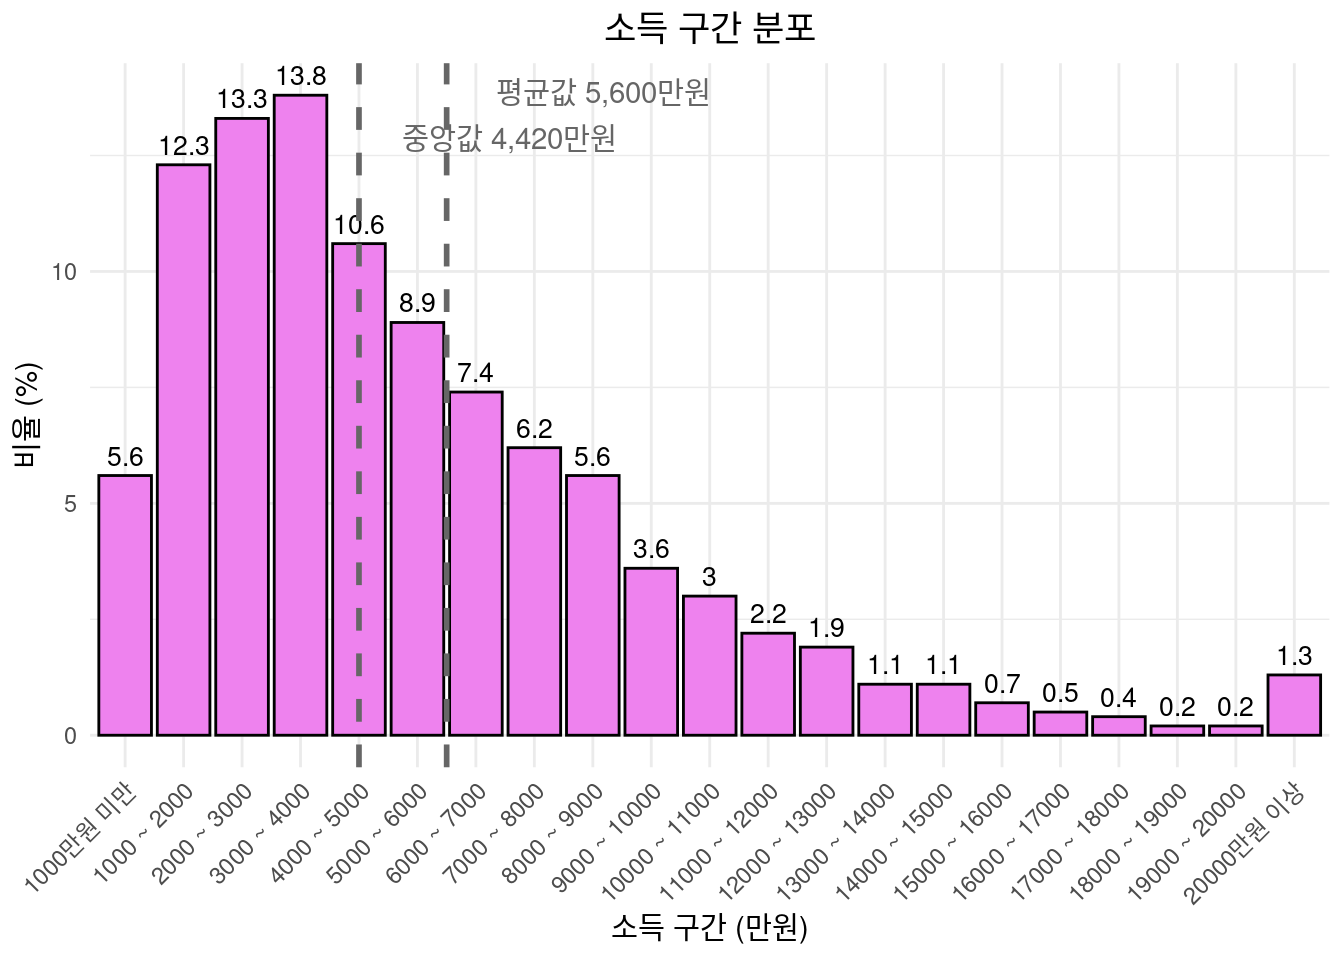
\includegraphics{01_descriptive_statistics/07_representative_value_files/figure-pdf/unnamed-chunk-3-1.pdf}

}

\end{figure}

\hypertarget{uxbcc0uxb7c9uxc758-uxd45cuxc900uxd654}{%
\chapter{변량의 표준화}\label{uxbcc0uxb7c9uxc758-uxd45cuxc900uxd654}}

변량 \(x\)의 평균을 \(\overline{x}\), 분산을 \({s_x }^2\)이라 할때 변량
y,z를 다음과 같이 정의

\[y = \frac{x - \overline{x}}{s_x}\] \[z = x - \overline{x}\] y를
`\textbf{x를 표준화한 변량}', z를 `\textbf{x를 중심화한 변량}' 이라고
함.

\begin{itemize}
\tightlist
\item
  표준화한 변량 y: 평균은 0, 분산은 1이 됨
\item
  중심화한 변량 z: 평균은 0이 됨
\end{itemize}

\hypertarget{uxd45cuxc900uxd654uxd55c-uxbcc0uxb7c9-uxb9ccuxb4e4uxae30}{%
\section{표준화한 변량
만들기}\label{uxd45cuxc900uxd654uxd55c-uxbcc0uxb7c9-uxb9ccuxb4e4uxae30}}

\href{https://sungileo.github.io/mine_statistics/01_descriptive_statistics/mean.html}{5장
평균, 분산, 표준편차}에서 살펴본 다음 데이터의 평균은 6, 표준편차는 10
이었습니다.

\begin{Shaded}
\begin{Highlighting}[]
\NormalTok{data }\OtherTok{\textless{}{-}} \FunctionTok{c}\NormalTok{(}\DecValTok{2}\NormalTok{,}\DecValTok{4}\NormalTok{,}\DecValTok{5}\NormalTok{,}\DecValTok{8}\NormalTok{,}\DecValTok{11}\NormalTok{)}
\FunctionTok{cat}\NormalTok{(data, }\StringTok{"}\SpecialCharTok{\textbackslash{}n}\StringTok{"}\NormalTok{,}
    \StringTok{"평균 : "}\NormalTok{, }\FunctionTok{mean}\NormalTok{(data), }\StringTok{"}\SpecialCharTok{\textbackslash{}n}\StringTok{"}\NormalTok{,}
    \StringTok{"분산 : "}\NormalTok{, }\FunctionTok{mean}\NormalTok{((data}\SpecialCharTok{{-}}\FunctionTok{mean}\NormalTok{(data))}\SpecialCharTok{**}\DecValTok{2}\NormalTok{))}
\end{Highlighting}
\end{Shaded}

\begin{verbatim}
2 4 5 8 11 
 평균 :  6 
 분산 :  10
\end{verbatim}

데이터를 표준화하려면 편차를 표준편차로 나눈다. 다음과 같다.

\[-\frac{4}{\sqrt{10}}, -\frac{2}{\sqrt{10}}, -\frac{1}{\sqrt{10}},\frac{2}{\sqrt{10}}, \frac{5}{\sqrt{10}}  \]

\begin{Shaded}
\begin{Highlighting}[]
\NormalTok{data\_std }\OtherTok{\textless{}{-}}\NormalTok{ (data }\SpecialCharTok{{-}} \FunctionTok{mean}\NormalTok{(data))}\SpecialCharTok{/}\FunctionTok{sd}\NormalTok{(data)}
\FunctionTok{cat}\NormalTok{(data\_std, }\StringTok{"}\SpecialCharTok{\textbackslash{}n}\StringTok{"}\NormalTok{,}
    \StringTok{"표준화된 데이터의 평균 : "}\NormalTok{, }\FunctionTok{mean}\NormalTok{(data\_std), }\StringTok{"}\SpecialCharTok{\textbackslash{}n}\StringTok{"}\NormalTok{,}
    \StringTok{"표준화된 데이터의 분산 : "}\NormalTok{, }\FunctionTok{sd}\NormalTok{(data\_std))}
\end{Highlighting}
\end{Shaded}

\begin{verbatim}
-1.131371 -0.5656854 -0.2828427 0.5656854 1.414214 
 표준화된 데이터의 평균 :  -2.218278e-17 
 표준화된 데이터의 분산 :  1
\end{verbatim}

\begin{Shaded}
\begin{Highlighting}[]
\FunctionTok{mean}\NormalTok{(}\FunctionTok{scale}\NormalTok{(data))}
\end{Highlighting}
\end{Shaded}

\begin{verbatim}
[1] -2.218278e-17
\end{verbatim}

평균이 0, 분산이 1이라는 것을 확인할 수 있다.

\begin{itemize}
\tightlist
\item
  평균이 정확히 0이 아닌 이유

  \begin{enumerate}
  \def\labelenumi{\arabic{enumi}.}
  \tightlist
  \item
    컴퓨터의 부동소수점 연산으로 인한 작은 오차
  \item
    과학적 표기법으로 표현된 매우 작은 수
  \item
    이 값은 실질적으로 0으로 간주할 수 있음
  \end{enumerate}
\end{itemize}

또한 변량을 1차식으로 변환해도 표준화한 값은 변하지
않는다.\textless\textgreater{}

\part{상관 관계}

\hypertarget{summary}{%
\chapter{Summary}\label{summary}}

In summary, this book has no content whatsoever.

\begin{Shaded}
\begin{Highlighting}[]
\DecValTok{1} \SpecialCharTok{+} \DecValTok{1}
\end{Highlighting}
\end{Shaded}

\begin{verbatim}
[1] 2
\end{verbatim}



\end{document}
